\chapter{Ievads}
Ievadā ir jāietver:

\begin{itemize}
\item temata aktualitātes pamatojums;
\item darba mērķis;
\item darba mērķa sasniegšanai veicamo uzdevumu formulējums;
\item izmantojamo pētīšanas metožu un paņēmienu uzskaitījums;
\item literatūras un avotu grupu uzskaitījums (piemēram, speciālā ekonomiskā literatūra, valsts statistikas dati, nepublicētie materiāli no uzņēmuma arhīva u.c.);
\item darba struktūras apraksts;
\item pētījuma temata un perioda norobežojums (ja tas nepieciešams).
\end{itemize}

Mašīnmācīšanās algoritmi ir kļuvuši par neatņemamu sastāvdaļu programmatūras izstrādātājiem un kompānijām, kas savas aplikācijas grib padarīt "gudras". Lai arī cik, mūsdienās, šis jēdziens ir kļuvis populārs, oficiāla mašīnmācīšanās definīcija nav noteikta. Visvienkāršākais mašīnmācīšanās pielietojums ir apstrādāt datus, mācīties no tiem un no iegūtajiem rezultātiem pieņemt lēmumus vai veikt minējumus reālās pasaules problēmu risināšanai. Tā vietā, lai manuāli veidotu programmatūras risinājumus, kas veic kādu uzdevumu, tiek apmācīti datori vai citas ierīces, izmantojot lielus datu apjomus. 
\section{Mašīnmācīšanās pamatjēdziens}
Pasaulē ir daudz un dažādi mašīnmācīšanās algoritmi un katru dienu tiek publicēti simtiem jaunu algoritmu. Tos var sagrupēt pēc apmācības veida (vadītā apmācība (\textit{supervised learning}), nevadītā apmācība (\textit{unsupervised learning}), pusvadītā apmācība (\textit{semi-supervised learning})) kā arī pēc formas vai funkcijas līdzībām (klasifikācija, regresija, lēmumu koki (\textit{decision trees}), klasterēšana (\textit{clustering}), dziļā mašīnmācīšanās (\textit{deep learning})). Neatkarīgi no apmācības veida vai pielietojuma, visas mašīnmācīšanās algoritmu kombinācijas sastāv no klasifikatoriem (atbalsta vektora mašīna, lēmuma koki, neironu tīkli), vērtēšanas funkcijām (varbūtības funkcijas, robežfunkcijas, izmaksu funkcija) un optimizācijas funkcijām (mantkārīgā meklēšana, nepārtrauktās optimizācijas metodes (\textit{continuous optimization})). Izmantojot šīs sastāvdaļas, mašīnmācīšanās algoritmu pamata mērķis ir būt spējīgam funkcionēt ne tikai ar apmācībā piedāvātajiem datiem, bet arī spēt darboties ar datiem, ar kuriem algoritms nav saskāries. 

Atkarībā no veicamā uzdevuma, ir dažādi veidi kā panākt, lai datori vai jebkura cita ierīce mācās, sākot ar visparastākajiem lēmumu kokiem, beidzot ar ģenētiskajiem algoritmiem un mākslīgajiem neironu tīkliem. Lēmumu koki atspoguļo reālās dzīves koka struktūru un tos izmanto gan klasifikācijas, gan regresijas problēmu risināšanā. Analizējot datus, lēmumu kokus var izmantot, lai vizuāli aprakstītu lēmumus un lēmumu pieņemšanu. Mašīnmācīšanās gadījumā, lēmumu kokus apraksta kā klasifikācijas kokus vai regresijas kokus (\textit{CART - Classification and Regression Trees}), atkarībā no veicamā uzdevuma.  Galvenā šo koku doma ir audzēt zarus, pieņemot lēmumus, kuras koka īpašības izvēlēties, zinot apstāšanās nosacījumu \cite{dectree}. Lai gan lēmumu koki nav vispopulārākais mašīnmācīšanās veids, taču tas ir pielietots klasifikācijas problēmu risināšanai dotajos pētījumos \cite{dectreepaper}\cite{pal2003assessment}.

Ģenētiskie algoritmi ir vēl viens algoritmu veids, kuru ir vērts izcelt. Tie ir algoritmi, kuri tiek izveidoti, balstoties uz notikumiem, kurus novēro dabīgajos evolūcijas procesos. Datorzinātnē ģenētiskie algoritmi ir optimizācijas algoritmi, kuri prot patstāvīgi apgūt jaunu informāciju, balstoties uz evolūcijas jēdzieniem kā dabīgā atlase un ģenētika. Ģenētisko algoritmu pamatideja ir simulēt Čārlza Dārvina piedāvāto teorēmu "izdzīvo stiprākais". Risinot problēmu, ģenētiskais algoritms saglabā tikai spēcīgākos indivīdus katrā paaudzē. Šie indivīdi sacenšas par resursiem un iespēju veidot nākamo paaudzi. Jaunās paaudzes tiek veidotas izvēloties vecākus no iepriekšējās paaudzes, veicot \textit{crossover} operāciju un mutāciju. Spēcīgākie indivīdi katrā paaudzē izveidos vairāk pēcnācēju nekā vājie indivīdi, tādējādi katra nākamā indivīdu paaudze kļūs labāka, galu galā iegūstot labāko rezultātu problēmas risināšanai. Beigu nosacījumu nosaka pirms algoritma izpildes, parasti, tiek noteikts paaudžu skaits vai kāds labāko indivīdu rezultātu slieksnis, kuru pēcnācēju paaudze pārsniedz. Ģenētiskie algoritmi gan nespēj risināt klasifikācijas problēmas, bet tos var lietot kā optimizācijas funkciju \cite{genopti} vai kā kārtošanas algoritmu \cite{deb2000fast}. Lai rēķinātu neironu tīklu svarus, var izmantot ģenētiskos algoritmus. \cite{genalg}
\begin{figure}[h]%
	\centering
	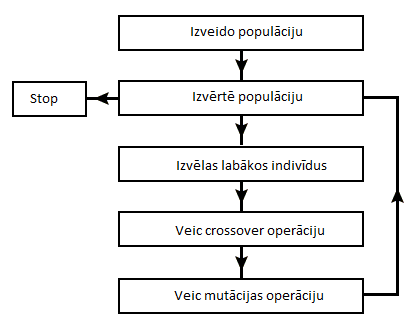
\includegraphics[height=6cm]{images/gen-algo-bilde.png} %
	\caption{Ģenētisko algoritmu modelis}%
	\label{fig:example}%
\end{figure}

Mākslīgie neironu tīkli ir viena no populārākajām mašīnmācīšanās izmantotajām metodēm. Tas ir neapstrādāts elektronisks modelis, kas balstīts uz smadzeņu bioloģisko neironu tīklu. Var teikt, ka šāda neironu tīkla modelis, līdzīgi kā smadzenes, mācās no pieredzes. Teorētiski, šādu smadzeņu modelēšana, paredz, ka šāds mašīnmācīšanās risinājums, neprasa dziļas tehniskas zināšanas bioloģijā vai datorzinātnē, bet ir jāspēj tīklu izveidot pareizi kopā saliekot vairākas slāņu kārtas. Šādas, bioloģijas iedvesmotas metodes uzskata par nākamo lielo soli datorzinātnes industrijā.\cite{staff} \par
Iedziļinoties mākslīgo neironu tīklu uzbūvē, neironu tīkls sastāv no daudz, savstarpēji savienotiem mezgliem, kur katrs no mezgliem veic kādu matemātisku operāciju. To, ko atgriež katrs mezgls, nosaka matemātiskā operācija, ko šis mezgls veic kā arī citi parametri, kas specifiski šim mezglam. Šie mezgli galu galā tiek grupēti un šos mezglu grupējumus sauc par slāņiem (no ang. val. - \textit{layer}). \par
Mākslīgie neironu tīkli satur sava veida "mācīšanās likumus", kas ir process, kad tiek mainīti mezglu savienojumu svari atkarībā no informācijas ievadē. 
Kad neironu tīkls ir apmācīts tik tālu, ka lietotājs ir apmierināts, tad tīklam var sākt piedāvāt datus, kuri tad iziet cauri visiem slāņiem, tādā veidā turpinot mācības uz sākumā izveidotā modeļa bāzes. Neironu tīklus ir arī iespējams pārtrenēt, kas nozīmē, ka tīkls atpazīst tikai vienu ienākošo datu tipu. Ja tā notiek, tad mācīšanās vairs nav iespējama. Mākslīgos neironu tīklus izmanto dažādu problēmu risināšanai, piemēram, rakstu zīmju atpazīšanai \cite{nnchars}, attēlu kompresēšanai \cite{dony1995neural} vai pat akciju tirgus analizēšanai \cite{kimoto1990stock}. Šī darba nolūkos autors neironu tīklus izmantos dziļajai apmācībai.
\begin{figure}[h]%
	\centering
	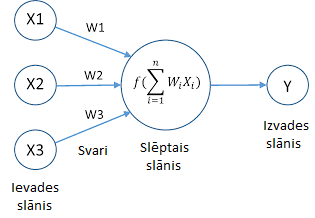
\includegraphics[height=5cm]{images/neironutikls.png} %
	\caption{Vienkāršs neironu tīkla modelis}%
	\label{fig:example}%
\end{figure}
\section{Dziļā mašīnmācīšanās}
Mašīnmācīšanās no dziļās mašīnmācīšanās atšķiras ar to, ka mašīnmācīšanās ir sarežģīti izmantot ļoti lielas datu kopas, taču ar dziļās apmācības metodēm tas ir iespējams. Dziļās mašīnmācīšanās metodes atgriež jebkādas vērtības sākot ar skaitliskām vērtībām, beidzot ar elementiem kā attēli, teksts vai skaņa, taču parastās mašīnmācīšanās metodes spēj atgriezt tikai skaitliskas vērtības kā, piemēram, klasifikācijas indeksu vai kādas funkcijas rezultātu. Mašīnmācīšanās izmanto dažādus automatizētus algoritmus, kas iemācās modeļa funkcijas un paredz nākotnes darbības no padotajiem datiem, kamēr dziļā apmācībā izmanto neironu tīklus, kas laiž datus caur daudz apstrādes slāņiem, lai izšķirtu datu īpašības. Lielākā atšķirība, pēc autora domām, starp mašīnmācīšanos un dziļo mašīnmācīšanos ir tajā, ka dziļās mašīnmācīšanās metodes automātiski datos atrod svarīgās īpašības, kamēr mašīnmācīšanās algoritmos šīs īpašības ir manuāli jānorāda. 
\begin{figure}[h]%
	\centering
	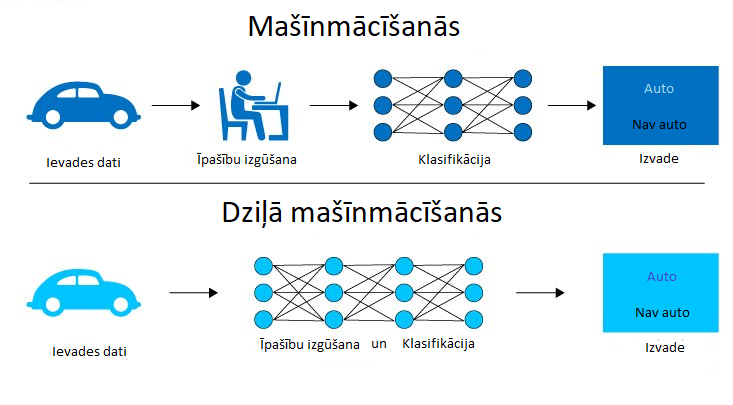
\includegraphics[height=7cm]{images/deeplearning.png} %
	\caption{Mašīnmācīšanās un dziļās mašīnmācīšanās salīdzinājums}%
	\label{fig:example}%
\end{figure}
Dziļā mašīnmācīšanās ļauj apmācīt matemātiskus modeļus, kas izveidoti no vairākiem datu apstrādes slāņiem, ar datiem, kas attēloti kā vairāku līmeņu abstrakcija (pētamā objekta galveno īpašību izdalīšana un mazsvarīgu aspektu ignorēšana). Šīs metodes ir uzlabojušas jaunākās tehnoloģijas balss atpazīšanā, objektu atpazīšanā attēlos, objektu detektēšanā. Dziļā mašīnmācīšanās, izmantojot atpakaļdatošanas algoritmus, sarežģītās datu kopu struktūrās meklē kā datoram vai jebkurai citai ierīcei būtu jāmaina iekšējie parametri starp tīklu slāņiem.

Īpašību apmācība ir metožu kopums, kas atļauj ierīcei padot neapstrādātus datus un automātiski iegūt īpašības, kas nepieciešamas, lai veiktu detektēšanu vai klasifikāciju. Dziļās mašīnmācīšanās metodes ir īpašību apmācības metodes ar vairākiem īpašību slāņiem, kurus iegūst apvienojot vienkāršus, taču nelineārus modeļus, kur katrs modelis pārveido īpašību no viena līmeņa uz augstāku, abstraktāku līmeni. Veicot pietiekami daudz šādus pārveidojumus, algoritmiem ir iespējams iemācīties ļoti sarežģītas darbības.\cite{deepnet} Darba ietvaros, datu klasifikācijai tiks izmantots konvolūciju neironu tīkls (\textit{CNN}), kas ir dziļās mašīnmācīšanās tips.

\section{Konvolūcijas neironu tīkli}
Konvolūcijas neironu tīkli (turpmāk \textit{CNN}) ir izveidoti, lai apstrādātu datus, kas ievadei padoti kā vairāki masīvi, piemēram, divdimensiju masīvi, kas satur pikseļu intensitātes vairākos krāsu kanālos (attēls). Vairākus datu veidus vienkāršojot, tos var izteikt kā masīvus: viendimensijas masīvs priekš signāliem vai skaitļu rindām, divdimensiju masīvi attēliem vai audio spektogrammām un trīsdimensiju masīvs video. Vislabāko rezultātu CNN tīklu veidi sasniedz risinot objektu detektēšanas \cite{li2015convolutional}\cite{matsugu2003subject}, segmentācijas \cite{long2015fully} vai klasifikācijas problēmas \cite{classif}\cite{krizhevsky2012imagenet}\cite{jia2014caffe}. Šī darba ietvaros CNN tiks izmantots objektu klasifikācijai.

\subsection{Tīklu slāņi}
Līdzīgi parastajiem neironu tīkliem arī konvolūciju neironu tīkli ir izveidoti no vairākiem slāņiem. CNN ir sarežģītāka struktūra kā parastam neironu tīklam. Vienkārša konvolūciju neironu tīkla arhitektūra sastāv no vairākiem, secīgi novietotiem slāņiem, kurus var izdalīt pa tipiem: konvolūcijas slānis (no kurienes arī rodas tīkla nosaukums), nelinearitātes slānis jeb aktivizācijas slānis, apvienošanas slānis un pilnīgi savienotais slānis (līdzīgi kāds tiek izmantots parastajos neironu tīklos). 
\subsubsection{Konvolūcijas slānis}
Konvolūcijas slānis ir CNN galvenā sastāvdaļa. Kā jau no nosaukuma var noprast, konvolūcijas slānī tiek veikta konvolūcijas operācija. Tiek izvēlēts filtrs (kernelis), un šis filtrs tiek pārvietots pāri masīvam (kas var būt gan attēls, gan audio, gan video) un katrā pozīcijā veic konvolūcijas operāciju. No konvolūcijas operācijas iegūtās vērtības tiek saskaitītas un rezultātā iegūts viens skaitlis. Kad konvolūcijas operācija tiek veikta visam masīvam, tiek iegūts masīvs, ko sauc par īpašību karti (no angļu val. \textit{feature map}) un jo vairāk filtrus izmanto, jo dziļāks kļūst attēls. Izmantojot 32x32x3 ievades masīvu un 5x5x3 filtru (filtram jābūt tikpat dziļam, cik dziļš ir ievades masīvs, lai būtu iespējams veikt matricu reizinājumu) tiks iegūta 28x28x1 īpašību karte un jo vairāk filtri tiks pielietoti, jo dziļāka būs šī īpašību karte un vairāk īpašības būs iespējams atrast masīvā. 
\begin{figure}[h]%
	\centering
	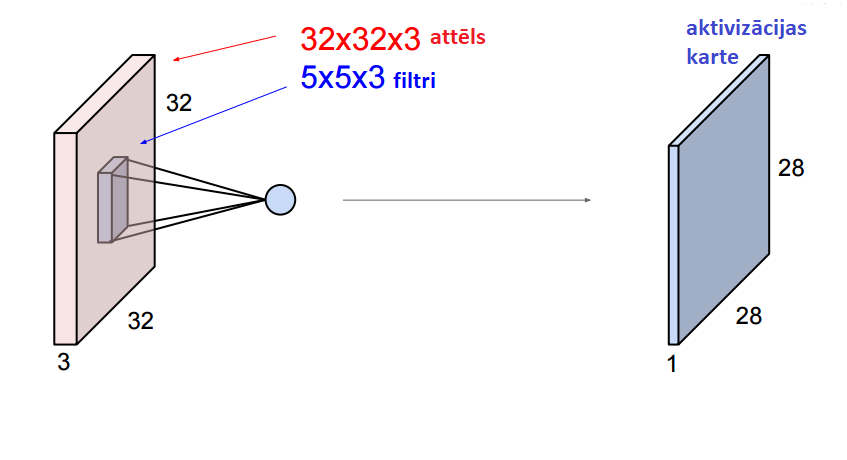
\includegraphics[height=4cm]{images/ActivationMap.png} %
	\caption{Konvolūcijas operācija pirmajā solī pielietojot 5x5 izmēra filtru}%
	\label{fig:example}%
\end{figure}
\\
~
\\
~
\\
~
\\

Šī īpašību karte satur informāciju par to kur atrodas minētās īpašības un cik labi šīs īpašības iedarbojas ar filtru, tādējādi norādot cik ļoti katrā masīva punktā atrodas ar filtru raksturotais elements. Pirms konvolūcijas operācijas veikšanas, ir nepieciešams izvēlēties trīs lielumus, kas ietekmēs īpašību karti:

\begin{itemize}
	\item \textbf{Dziļums} - atbilst filtru skaitam, kas izvēlēts konvolūcijas operācijas veikšanai. Ja ar masīvu tiks veikta konvolūcijas operācija ar trīs dažādiem filtriem, tad tiks atgrieztas trīs dažādas īpašību kartes, kuras būs apvienotas vienā trīs dimensiju masīvā ar dziļumu trīs.
	\item \textbf{Solis} - norāda par cik pikseļiem ievades masīvā pārvietosies filtra masīvs. Piemēram, ja konvolūcijas operāciju veic attēlam un solis ir divi, tad filtri neiet cauri katram pikselim, bet katram otrajam sākot no attēla augšējā kreisā stūra. Jo lielāks solis, jo mazākas būs īpašību kartes, kas ir noderīgi, ja tiek izmantoti lieli vai arī daudz filtru. Tādējādi, ir iespējams ietaupīt skaitļošanas resursus. 
	\item \textbf{Nulles-apdare} (no angļu val. \textit{zero-padding}) - tiek izmantota, ievades matricai pieliekot nulles vērtības ap robežām, lai šiem robežu elementiem būtu pilnībā iespējams pielietot filtrus. Nulles-apdares labās īpašības var izmantot arī lai mainītu īpašību kartes izmērus. Izmantojot nulles-apdari, šis process tiek dēvēts par plato konvolūciju (no angļu val. \textit{wide convolution}), bet nulles-apdares neizmantošanu sauc par šauro konvolūciju (no angļu val. \textit{narrow convolution}). 
	\begin{figure}[h]%
		\centering
		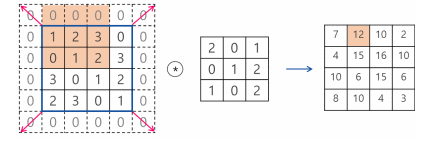
\includegraphics[height=2.5cm]{images/zero-padding.png} %
		\caption{Nulles-apdares piemērs \cite{zerpad}}%
		\label{fig:example}%
	\end{figure}
\end{itemize}
\subsubsection{Nelinearitātes slānis}
Nelinearitātes slānis konvolūciju neironu tīklos satur aktivizācijas funkciju, kas ņem no konvolūcijas operācijas atgriezto īpašību karti un izveido aktivizācijas karti. Aktivizācijas funkcija veic matricas elementu reizinājumu izmantojot saņemtos datus, kas nozīmē, ka tiek izvadīts tik pat liels masīvs, cik bija saņemts ievadē. Aktivizācijas funkciju tradicionāli implementē kā sigmoīdu vai hiperbolisku tangensa funkciju un tās galvenais mērķis ir novērst linearitāti. Nesenāki pētījumi gan norāda, ka konvolūcijas neironu tīklos rektificētas lineārās vienības (no angļu val. \textit{rectified linear units}) (ReLUs) strādā labāk kā tradicionālās aktivizācijas funkcijas \cite{nair2010rectified}. 
\begin{figure}[h]%
	\centering
	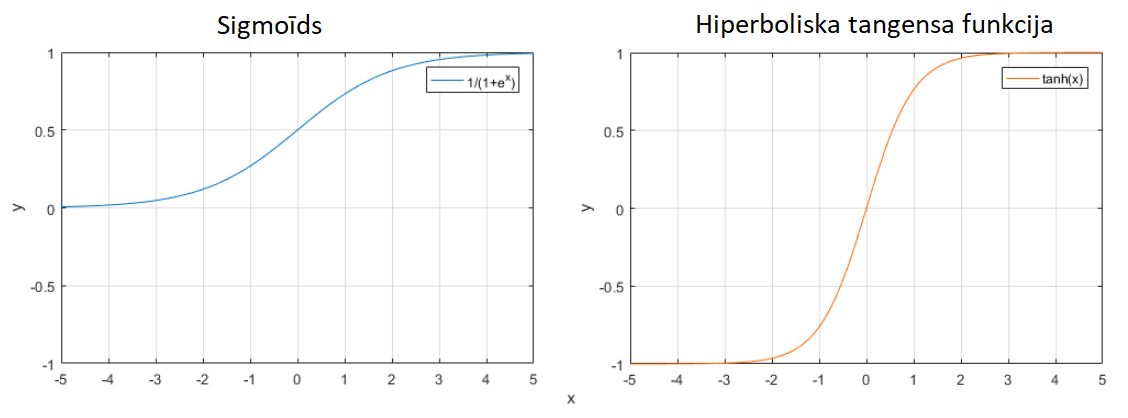
\includegraphics[height=4cm]{images/sigmoidhiperbol.png} %
	\caption{Sigmoīds un hiperboliskā tangensa funkcija ir populāri\\ izmantotas aktivizācijas funkcijas konvolūcijas neironu tīklos}%
	\label{fig:example}%
\end{figure}

Rektificētās lineārās vienības (ReLUs) ir speciāla implementācija, kas apvieno nelinearitātes un rektifikācijas slāņu (rektifikācijas slānis atgriež ievades datu elementu moduli) operācijas konvolūcijas neironu tīklos. Rektificēta lineāra vienība ir gabalveida (no angļu val. \textit{piecewise}) lineāra funkcija, kas definēta sekojoši:
\[ Y_i^{(l)} = max(0,Y_i^{(l-1)}) \]
\begin{figure}[h]%
	\centering
	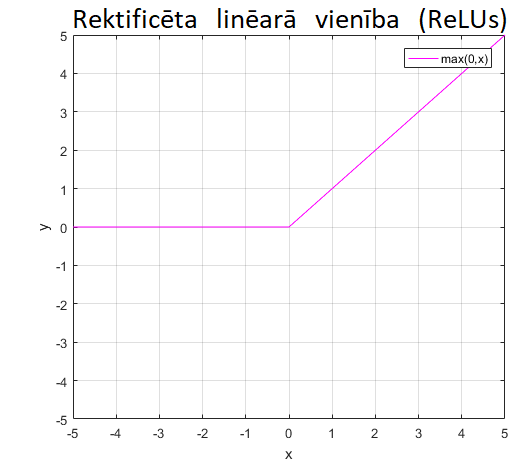
\includegraphics[height=4cm]{images/relu.png} %
	\caption{Rektificēta lineāra vienība}%
	\label{fig:example}%
\end{figure}

Konvolūcijas neironu tīklos, ReLUs ir trīs nozīmīgas priekšrocības pār tradicionālajām loģistikas funkcijām (sigmoīds) vai hiperboliskajām tangensa aktivizācijas funkcijām:
\begin{itemize}
	\item ReLUs efektīvi izplata gradientu, kas samazina iespēju saskarties ar gradienta izzušanas problēmu, kas ir parasta problēma dziļajās neironu tīklu arhitektūrās \cite{hochreiter1998vanishing}.
	\item Īpašības karšu negatīvās vērtības, rektifikācijas lineārā vienība pārveido par nullēm, tādējādi tiekot galā ar anulēšanas problēmu (no angļu val. \textit{cancellation problem}) kā arī izvadē iegūtā aktivizācijas karte saturēs daudz izsētāku vērtību apjomu. Šāds vērtību izkaisījums nodrošina stabilitāti gadījumā, ja ievadē notiek nelielas izmaiņas, piemēram, troksnis\cite{glorot2011deep}. 
	\item Ņemot vērā skaitļošanas sarežģītību, ReLUs sastāv no ļoti vienkāršām operācijām, kas nozīmē, ka šīs operācijas smagi neietekmē CNN veiktspēju, kas padara to implementēšanu konvolūcijas neironu tīklos ļoti efektīvu.
\end{itemize}
Šo priekšrocību dēļ, lielākā daļa jaunāko konvolūcijas neironu tīklu arhitektūru, piemēram, \cite{krizhevsky2012imagenet}\cite{DBLP:journals/corr/HeZR015}\cite{simonyan2014very}, izmanto tieši rektificētās lineārās vienības kā aktivizācijas funkciju nelinearitātes slānī.
\subsubsection{Apvienošanas slānis}
Apvienošanas slāņa (no angļu val. \textit{pooling layer}) galvenā funkcija ir samazināt aktivizāciju karšu dimensiju skaitu. Lai samazinātu iespēju pārlieku apmācīt tīklus (no angļu val. \textit{overfitting}) un samazinātu nepieciešamos skaitļošanas resursus, visbiežāk, šis slānis tiek pielietots pēc vairāk citu slāņu operāciju veikšanas (piemēram, pēc vairākiem konvolūcijas un aktivizācijas slāņiem). Apvienošanas operācijas mērķis ir saglabāt jau atrastās īpašības mazākā attēlojumā. Šis mērķis tiek sasniegts atmetot mazsvarīgos datus, lai iegūtu labāku telpisko izšķirtspēju. 

Apvienošanas slānī tiek definēts filtrs, kurš katrā operācijas solī tiks reducēts līdz vienai vērtībai. Līdzīgi kā konvolūcijas slānī, tiek izvēlēts solis pēc cik pozīcijām atkal tiks pielietots apvienošanas filtrs. Kad filtrs ir izmantots visām iespējamajām masīva pozīcijām, izvadē tiek iegūta telpiski samazināta aktivizācijas karte.

Visbiežāk izmantotās redukcijas metodes ir maksimumu apvienošana vai vidējās vērtības apvienošana. Maksimuma apvienošanas filtri meklē vislielāko vērtību filtra reģionā un atmet pārējās vērtības. Vidējās vērtības apvienošanas filtri saglabā filtr reģiona vidējo vērtību. Maksimuma apvienošana demonstrē spēju ātrāk konverģēt salīdzinājumā ar vidējās vērtības apvienošanu un citām metodēm, tāpēc to izmanto visbiežāk \cite{scherer2010evaluation}. 
\begin{figure}[h]%
	\centering
	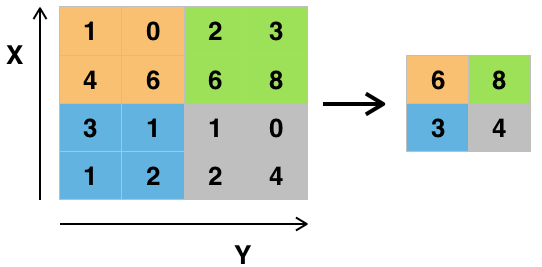
\includegraphics[height=3cm]{images/maxpool.png} %
	\caption{Vienkāršs maksimuma apvienošanas slāņa modelis \cite{maxpool}}%
	\label{fig:example}%
\end{figure}
\subsubsection{Pilnīgi savienotais slānis}
Pilnīgās savienošanas slāņa (no angļu val. \textit{fully connected layer}) galvenais uzdevums ir, izmantojot no iepriekšējiem slāņiem iegūto īpašību karti, sadalīt ievades datu masīvu pa klasēm, kas balstītas uz apmācībā izmantoto datu kopu. Papildu klasifikācijas funkcijai, pilnīgi savienotos slāņus ir vērts ievest tīklā, lai noskaidrotu īpašību karšu nelineārās kombinācijas. Šis slānis kā ievades datus saņem konvolūcijas, aktivizācijas vai apvienošanas slāņu izvadi un atgriež \textit{N} dimensiju vektoru, kur \textit{N} ir neironu tīklam piedāvāto klašu skaits. Šis klašu jeb atšķirīgu detektējamo objektu skaits ir jādefinē pirms tīkla apmācības. Iepriekš minētais vektors saturēs informāciju par to cik ļoti katrs aktivizācijas kartes elements korelē ar definētajām klasēm. Piemēram, ja tīklam ievadē ir padots attēls ar cilvēku, aktivizācijas kartē būs augstas vērtības īpašībām, kas raksturo, ka objektam ir divas rokas un divas kājas. Summējot no pilnīgi savienotā slāņa izvadē iegūtās varbūtības ir jāiegūst vērtība 1. To nodrošina \textit{Softmax} funkcija, ko izmanto kā aktivizācijas funkciju pilnīgi savienotajā slānī. \textit{Softmax} funkcijai kā ievades datus padod vektoru ar patvaļīgiem rezultātiem, kas iegūti pēc klasifikācijas un šī funkcija saspiež šīs vērtības vektorā, kur visas vērtības ir robežās no 0 līdz 1 un visa vektoru vērtību summa ir 1. \textit{Softmax} aktivizācijas funkcija ir definēta sekojoši:
\[f_j(z) = \frac{e^{z_j}}{\sum_k e^{z_k}} \]
Kur \textit{z} ir masīvs ar vērtībām, kas iegūtas pēc klasifikācijas.
\subsection{Tīklu arhitektūras}
Nav noteikts viens veids kādai ir jābūt pareizai konvolūcijas neironu tīkla struktūrai, taču ir pieņemts, ka konvolūcijas neironu tīkls vienmēr satur jau minētos tīkla slāņus. Mūsdienās, standarta CNN arhitektūru sāk aizvietot ar sarežģītākām tīklu arhitektūrām, kuras visbiežāk parastos četrus konvolūcijas neironu tīklu slāņus maina vietām un atkārto vairākas reizes. Izveidot pašam savu CNN struktūru nav sarežģīti, to pat var padarīt funkcionālu, taču, lai tas funkcionētu labāk kā jau esošās arhitektūras, ir nepieciešams ieguldīt daudz laika testēšanai un pētīšanai. Dotajā brīdī, ir pieejami tūkstošiem, un katru dienu parādās jaunas, konvolūcijas neironu tīklu arhitektūras, šī darba ietvaros ir vērts pieminēt dotās tīklu arhitektūras: \textit{AlexNet}, \textit{VGG Net}, \textit{GooGleNet} un \textit{ResNet}.

\subsubsection{AlexNet}

\textit{AlexNet} tīklu arhitektūru var uzskatīt par pirmo konvolūcijas neironu tīklu arhitektūru, kas uzrādija labus rezultātus, risinot objektu detektēšanas, klasifikācijas un lokalizācijas problēmas \cite{ILSVRC15}. Tā tika izveidota 2012. gadā un ir aprakstīta rakstā \textit{"ImageNet Classification with Deep Convolutional Networks"}\cite{krizhevsky2012imagenet}. 2012. gada ILSVRC (\textit{ImageNet Large-Scale Visual Recognition Challenge}) \textit{AlexNet} sacensībās uzrādīja tik labus rezultātus kā neviena CNN arhitektūra līdz šim \cite{ILSVRC15} un kopš šīm sacensībām CNN vispārīgi sāka gūt popularitāti objektu detektēšanā. 

Salīdzinājumā ar mūsdienu arhitektūrām, \textit{AlexNet} struktūra ir salīdzinoši vienkārša. Tīklā ir 5 konvolūcijas, apvienošanas slāņi un nelinearitātes slāņi un 3 pilnīgi savienotie slāņi. Nelinearitātes slānī tiek izmantota \textit{ReLU} aktivizācijas metode, jo testēšanas procesā, \textit{ReLU} apmācības laiki bija vairākas reizes mazāki, kā ierastajai hiperboliskajai tangensa aktivizācijas funkcijai. 
\begin{figure}[h]%
	\centering
	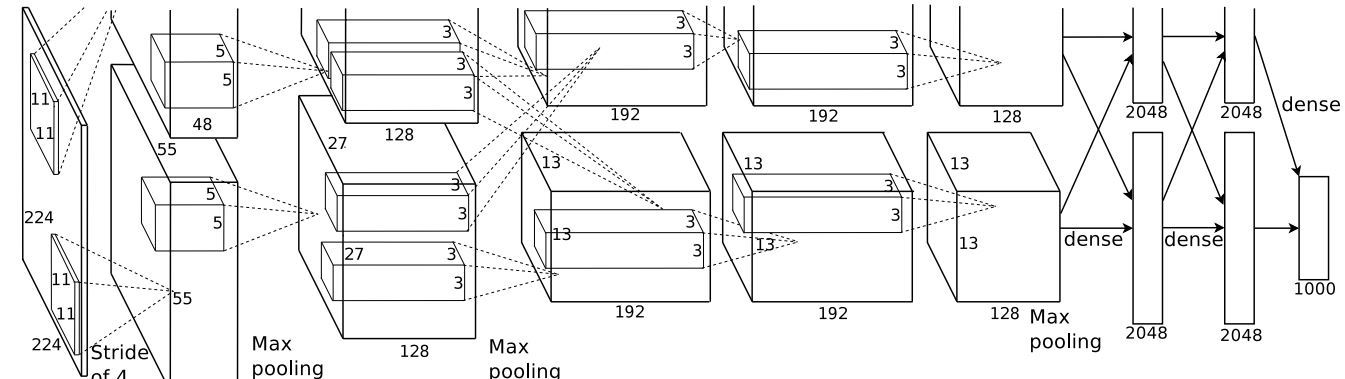
\includegraphics[height=4cm]{images/alexnet.jpg} %
	\caption{\textit{AlexNet} tīkla arhitektūra \cite{alexnetimage}}%
	\label{fig:example}%
\end{figure}
\subsubsection{VGG Net}
\textit{VGG Net} arhitektūra ir izveidota 2014. gadā un aprakstīta rakstā ar nosaukumu \textit{"Very deep convolutional networks for large-scale image recognition"}\cite{simonyan2014very}. Šīs arhitektūras galvenā īpašība ir vienkāršība un slāņu daudzums (no angļu val. \textit{depth}), saglabājot tīklu nesarežģītu. \textit{VGG Net} ir 19 slāņu konvolūcijas neironu tīkls, kas konvolūcijas slānī izmanto mazus, 3x3 izmēra filtrus ar soli 1 un 1 \textit{zero-padding} jeb nulles-apdares operāciju un apvienošanas slānī izmanto 2x2 filtrus ar soli 2.
Pēc tīkla arhitektūras autoru domām, lai gan 3x3 izmēru filtri ir mazi, divus filtrus ir iespējams apvienot (novietojot 2 konvolūcijas slāņus vienu pēc otra), simulējot 5x5 izmēra filtru un apvienojot 3 konvolūcijas filtrus tiks simulēts 7x7 filtrs. Vairāku filtru apvienošana dod iespēju iegūt lielāku filtra izmēru, saglabājot labās mazo filtru īpašības, piemēram, ar vairākiem konvolūcijas slāņiem, ir iespējams arī vairākas reizes pielietot \textit{ReLU} aktivizācijas funkciju. Izmantojot vairākus mazus filtrus, tīkls var iemācīties smalkākas, sarežģītākas īpašības būtiski neietekmējot skaitļošanas resursu izmantošanu.
\begin{figure}[h]%
	\centering
	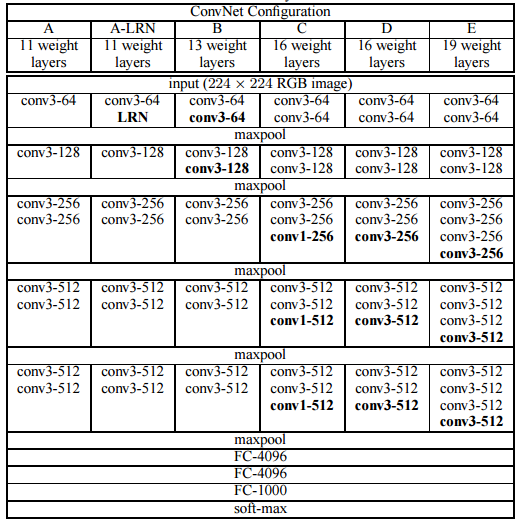
\includegraphics[height=7cm]{images/vggnet.png} %
	\caption{\textit{VGG Net} tīklu struktūras \cite{simonyan2014very}}%
	\label{fig:example}%
\end{figure}

\textit{VGG Net} arhitektūrā, pēc katra apvienošanas slāņa, konvolūcijas slāņos izmantotas filtru skaits dubultojas. Kā rezultātā datu telpiskais izmērs pēc konvolūcijas un apvienošanas slāņu operācijām samazinās, bet datu dziļums palielinās, kas ir rezultāts daudz filtru pielietošanai. Attēlā 1.10 ir parādīts, ka \textit{VGG Net} struktūra ir sadalīta blokos un katrā blokā konvolūcijas operācija, ar vienāda izmēra filtriem, tiek veikta vairākas reizes, lai iegūtu smalkākas īpašības.
\subsubsection{GoogLeNet}
Pretēji \textit{VGG Net} principam "vienkāršība un dziļums", \textit{GoogLeNet} arhitektūrai ir ļoti sarežģīta struktūra, kurā ir iebūvēti \textit{Inception} modeļi. \textit{GoogLeNet} 2015. gadā izveidoja kompānijas \textit{Google} pētnieki un aprakstīja tīkla arhitektūru rakstā "\textit{Going Deeper with Convolutions}" \cite{szegedy2015going}. \textit{GoogLeNet} arī uzvarēja 2014. gada ILSVRC sacensībās \cite{ILSVRC15}. Šī tīkla arhitektūra bija pirmā, kas novērsās no standarta metodēm: konvolūciju neironu tīklus kārtot slāņus secīgi, vienu pēc otra, piedāvājot slāņus kārtot paralēli.

\textit{GoogLeNet} arhitektūru sakārtojot secīgi, tā izmantotu milzīgus atmiņas apjomus un prasītu pamatīgus skaitļošanas resursus, taču, izmantojot \textit{Inception} modeļus, šo problēmu var samazināt.
\begin{figure}[h]%
	\centering
	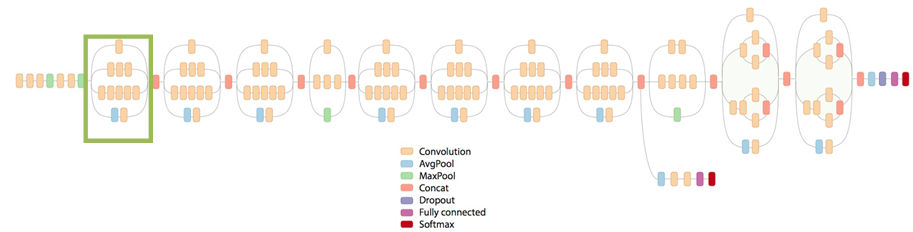
\includegraphics[height=4cm]{images/GoogLeNet2.png} %
	\caption{\textit{GoogLeNet} tīkla struktūra \cite{szegedy2015going}}%
	\label{fig:example}%
\end{figure}

Attēlā 1.11 var novērot, ka tīkla struktūra ir sadalīta moduļos (piemērs zaļā taisnstūrī) un šie moduļi satur blokus, kas ir novietoti paralēli viens otram. Katrs šis modelis ir \textit{Inception} modelis. Šis modulis ir kā vairāki konvolūcijas filtra ievades punkti, kurus apstrādā vienlaicīgi, paralēli, visus rezultātus pēc tam savieno, šādā veidā no katras ievades datu vienības tiek veikta vairāku līmeņu īpašību (\textit{feature}) izgūšana.

\begin{figure}[h]%
	\centering
	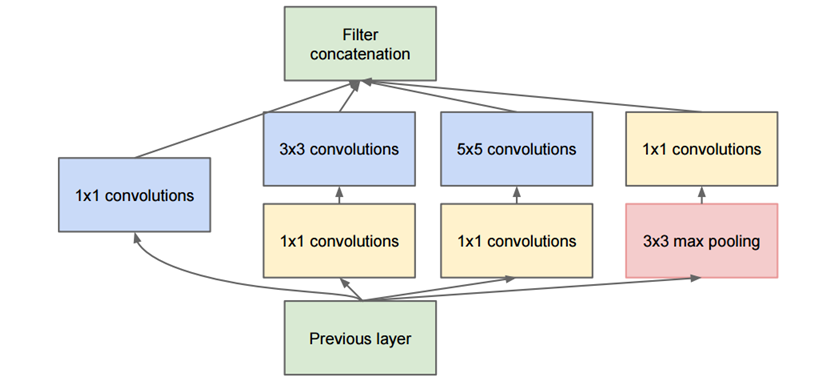
\includegraphics[height=4cm]{images/inception.png} %
	\caption{\textit{Inception} modelis \cite{szegedy2015going}}%
	\label{fig:example}%
\end{figure}

\subsubsection{ResNet}
No augstāk minēto arhitektūru aprakstiem, var izdarīt secinājumu, ka palielinot slāņu skaitu, palielināsies tīkla precizitāte (ja netiek pieļauta tīkla pār-apmācīšana (no angļu val. \textit{overfitting})). \textit{Microsoft} komandas, 2015. gadā izveidotā CNN arhitektūra ir 152 slāņu arhitektūra, kas uzstādīja jaunus rekordus klasifikācijā, detektēšanā un lokalizācijā, uzvarot 2015. gada ILSVRC sacensībās \cite{ILSVRC15}. 

Neskaitot lielo slāņu skaitu,    \textit{ResNet} tīklu struktūra no pārējām, jau minētajām, arhitektūrām atšķirt tas, ka \textit{ResNet} sastāv no "atlikumu blokiem" (no angļu val. \textit{residual blocks}). Šo bloku galvenā doma ir saglabāt tajā padoto informāciju un pievienot to izejošajai informācijai, nevis pilnībā aizmirst ievades datus kā tas notiek citās arhitektūrās \cite{he2016deep}. 

\begin{figure}[h]%
	\centering
	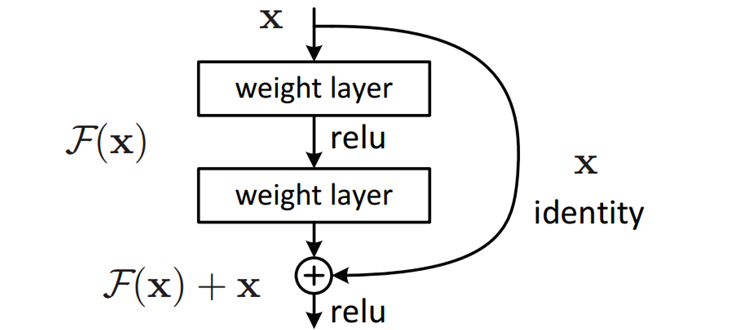
\includegraphics[height=4cm]{images/resnet.png} %
	\caption{\textit{ResNet} atlikumu bloks \cite{he2016deep}}%
	\label{fig:example}%
\end{figure}
\subsection{Tīklu apmācība}
Vispārīgu konvolūcijas neironu tīklu apmācību, pieņemot, ka ievades dati ir attēli un ir definētas 4 klases, var aprakstīt sekojošos soļos:
\begin{enumerate}
	\item solis - Tiek inicializēti visi filtri un tīkla parametri/svari ar gadījuma vērtībām.
	\item solis - Tīkls saņem apmācības datus, šie dati iziet cauri visiem CNN slāņiem (konvolūcijas, nelinearitātes un apvienošanas) un atrod katras klases varbūtības.
	\item solis - Tiek aprēķināta kļūda izvades slānī. 
	\item solis - Izmantojot atgriezenisko saiti, tiek aprēķināti kļūdu gradientu, ņemot vērā visus tīklā iegūtos svarus. Pēc tam izmanto gradienta nolaišanos (no angļu val. \textit{gradient descent}), lai atjaunotu visas filtra vērtības/svarus, tādējādi minimizējot kļūdu izvades slānī. Ja iegūtās varbūtības pirms šī soļa bija [0.2, 0.4, 0.1, 0.3], tagad iegūtās varbūtības jau var būt [0.1, 0.1, 0.7, 0.1], kas jau ir tuvāk mērķa vektoram [0, 0, 1, 0]. Tas nozīmē, ka tīkls ir pareizi iemācījies klasificēt šo attēlu, mainot svaru / filtru vērtības tā, ka kļūda izvades slānī samazinājās. Parametri kā filtru skaits, filtru izmēri, tīkla arhitektūra paliek nemainīgi visā tīkla apmācību garumā, tikai filtru un svaru vērtības mainās.
	\item solis - Atmešanas tehnika (no angļu val. \textit{dropout}). Lai gan ne visas tīklu arhitektūras izmanto atmešanas tehniku, to ir vērts pieminēt, jo tas ir veids kā cīnīties ar pār-apmācīšanu (no angļu val. \textit{overfitting}). Apmešanas tehnikas galvenā doma ir apmācību procesā neatjaunot svaru vērtības atsevišķiem tīkla mezgliem (no angļu val. \textit{nodes}). Katram mezglam tiek norādīta varbūtība ar kādu var gadīties, ka tā svari netiek atjaunoti.
	\item solis - Atkārto 2., 3., 4. un 5. soli ar visiem datu kopā esošajiem attēliem.
	\item solis - Apstāšanās nosacījums. Teorētiski, konvolūciju neironu tīklu apmācīšanas process var būt bezgalīgs, taču tā ir iespējams saskarties ar tīkla pār-apmācīšanu. Lai izvairītos no šīs problēmas ir nepieciešams sekot līdzi apmācības precizitātei (norāda cik labi modelis ir iemācījies atpazīt ievades datus) un validācijas precizitātei (norāda cik vispārīgi tīkls atpazīst datus). Ja apmācības precizitāte palielinās, vienlaicīgi validācijas precizitātei samazinoties, ir iespējams, ka notiek pār-apmācība. Ja pār-apmācība nenotiek, ierasta prakse ir orientēties pēc kļūdas funkcijas vai iterāciju skaita.
\end{enumerate}

Augstāk minētie soļi apmāca konvolūcijas neironu tīklu, kas nozīmē, ka visi svari un tīkla parametri ir optimizēti, lai pareizi klasificētu datu kopā esošos attēlus. Kad tīklam tiek padots jauns, līdz šim neredzēts attēls (attēls, kas netika izmantots apmācību laikā), ar to tiks veikts 2. solis no augstāk minētā saraksta un tiks atgriezta varbūtība ar kādu attēlā esošie objekti pieder katrai klasei. Ja datu kopa ir pietiekami liela un tīkls ir labi apmācīts, tas spēs jaunos attēlus sadalīt pareizās kategorijās. 